% arXiv preprint template for biomedical / computational biology papers (IMRaD)
% Layout: arxiv.sty by George Kour (MIT). Header/footer: fancyhdr.sty (LPPL), bundled locally.
% Compile: python .agents/skills/arxiv-preprint/scripts/build.py manuscript --bib library/references.bib
\documentclass{article}

\usepackage{arxiv}               % bundled in this folder
\usepackage[utf8]{inputenc}
\usepackage[T1]{fontenc}
\usepackage{lmodern}
\usepackage{url}
\usepackage{booktabs}            % \toprule \midrule \bottomrule
\usepackage{amsmath,amsfonts}
\usepackage{graphicx}
\usepackage{float}
\usepackage{microtype}
\usepackage[numbers,sort&compress]{natbib}   % or [authoryear,round] for author-year citations
\usepackage[hidelinks]{hyperref}

\graphicspath{{figures/}}

\begin{document}

% Sections are numbered by writing order (01 to 07) and included here in reading order:
% 06-title.tex — Finalized Title, Running Head, and Authors

\renewcommand{\headeright}{Preprint}
\renewcommand{\undertitle}{Preprint}
\renewcommand{\shorttitle}{Longitudinal Reanalysis of Auto-FMT Microbiome Trajectories}

\title{Longitudinal Reanalysis of Gut Microbiome Trajectories Following Autologous Fecal Microbiota Transplantation in Hematopoietic Cell Transplant Recipients: A QIIME 2 Methodological Case Study}

\author{
  Author Name\textsuperscript{1}\thanks{Corresponding author: \texttt{author@institution.edu}} \\[2pt]
  \textsuperscript{1}Department, Institution, City, Country
}

\date{}   % arXiv adds its own submission date
\maketitle

% 05-abstract.tex — Structured Abstract & Keywords
% arXiv limit: abstract field <= 1,920 characters.

\begin{abstract}
\textbf{Background:} Conditioning and antibiotics during allogeneic hematopoietic cell transplantation (allo-HCT) severely deplete gut microbial diversity. Autologous fecal microbiota transplantation (auto-FMT) aims to restore baseline microbiota, but longitudinal evaluation is complicated by repeated-measures correlation, irregular sampling, and single-step rarefying.

\textbf{Methods:} Using QIIME 2 (v2026.7), we reanalyzed 16S rRNA V4 data from trial NCT02269150. Filtering of 12,546 samples isolated trial participants across days $-10$ to $+70$ post-HCT, removed singleton and organellar features, and rarefied libraries at 10,000 reads, retaining 356 samples (2,422 ASVs) from 24 patients (10 control, 150 samples; 14 auto-FMT, 206 samples). A standalone 41-sample dataset demonstrated DADA2 denoising. Richness was evaluated via Kruskal-Wallis tests and linear mixed-effects (LME) modeling (\texttt{observed\_features} $\sim$ \texttt{day-relative-to-fmt} $\times$ \texttt{autoFmtGroup} with patient random intercepts), and temporal indicator genera via random forest regression.

\textbf{Results:} Observed ASV richness fell sharply post-HCT ($H = 70.58$, $q = 1.33 \times 10^{-16}$). Pooled cross-sectional testing showed no group difference ($H = 1.29$, $p = 0.256$). Conversely, LME modeling estimated a control decline of $-0.859$ ASVs/day ($p < 0.001$) and an auto-FMT interaction of $+0.560$ ASVs/day (95\% CI $[0.104, 1.015]$, $p = 0.016$; net slope $-0.299$ ASVs/day), though the REML optimizer did not converge. Random forest regression predicted post-HCT week ($R^2 = 0.319$, $r = 0.565$, $p = 2.37 \times 10^{-7}$), led by \textit{Enterococcaceae} (0.124), \textit{Clostridium} (0.109), \textit{Enterococcaceae Incertae Sedis} (0.089), and \textit{Lachnospiraceae} (0.087).

\textbf{Conclusions:} Longitudinal mixed modeling detects trajectory differences masked by cross-sectional pooling, but small unbalanced cohorts, LME non-convergence, single-slope models, single rarefying, and unverified strain engraftment require specialized longitudinal tools.
\end{abstract}

\keywords{autologous fecal microbiota transplantation \and hematopoietic cell transplantation \and gut microbiome \and longitudinal mixed-effects model \and QIIME 2}

% 03-introduction.tex — Introduction
% Structure: Clinical background & auto-FMT -> Methodological challenges in longitudinal microbiome analysis -> Study aims & research questions.

\section{Introduction}

Allogeneic hematopoietic cell transplantation (allo-HCT) is a potentially curative therapy for hematologic malignancies and bone marrow failure syndromes, yet the conditioning chemotherapy, radiation, and broad-spectrum antibiotics administered during the peri-transplant period severely disrupt the host gut microbiome. This acute ecological injury is characterized by a steep collapse in microbial richness and the opportunistic domination of the intestinal lumen by pathobionts such as \textit{Enterococcaceae}, and this loss of gut microbiota diversity during allo-HCT is associated with increased mortality \citep{taur2018reconstitution}. Autologous fecal microbiota transplantation (auto-FMT)---in which a patient's own pre-treatment stool is cryopreserved prior to conditioning and reinfused following antibiotic cessation and hematopoietic engraftment---offers a targeted strategy to restore baseline microbial diversity without exposing immunocompromised recipients to third-party donor pathogens \citep{herman2024assessing,herman2024assessingb}. In a randomized trial of 25 allo-HCT patients (14 auto-FMT, 11 control), auto-FMT was reported to boost microbial diversity and reestablish the intestinal microbiota composition present before antibiotic treatment and transplantation \citep{taur2018reconstitution}. However, determining whether and how auto-FMT alters post-transplant microbiome trajectories requires analytical frameworks capable of separating intervention-associated recovery from the massive background temporal shifts induced by transplantation itself.

Evaluating microbiome interventions in longitudinal clinical cohorts presents several interrelated statistical and bioinformatic challenges. First, clinical microbiome trials collect repeated fecal specimens from the same individuals across irregular follow-up schedules; pooling these observations into cross-sectional rank tests violates sample independence (pseudoreplication), inflates false discovery rates, and allows large pre- versus post-transplant variance to mask between-group trajectory differences \citep{herman2024assessingb,zhou2021linda,zhang2026bayesian}. Second, standard diversity workflows commonly normalize library sizes via a single random subsampling without replacement (rarefying) to a fixed read threshold, a practice that discards valid sequencing reads and excludes low-depth specimens that often correspond to the most severely depleted post-antibiotic states \citep{mcmurdie2013waste,raspet2024facilitating}. Third, while linear mixed-effects (LME) models account for within-subject correlation through patient-specific random effects, standard restricted maximum likelihood (REML) optimizers frequently encounter convergence failures under small sample sizes and unbalanced designs \citep{barrera2025stochastic}, and single-slope linear specifications across pre- and post-intervention time points can oversimplify piecewise or time-varying recovery dynamics \citep{fontaine2026locally}. Finally, general diversity recovery or temporal taxonomic shifts identified by supervised machine learning do not by themselves establish the engraftment of reinfused baseline strains \citep{herman2024assessing,herman2024assessingb} or correct for the compositional nature of sequencing count data \citep{zhou2021linda}.

In this study, we performed a structured longitudinal reanalysis of 16S rRNA amplicon sequencing data from the randomized auto-FMT trial NCT02269150 (356 retained fecal samples from 24 allo-HCT patients across days $-10$ to $+70$ relative to transplantation) using the QIIME 2 platform. Specifically, we addressed three research questions: (1) how gut microbial richness and community structure change across the peri-transplant timeline; (2) whether longitudinal LME modeling reveals a divergence in richness trajectories between the auto-FMT and control arms that is obscured when samples are pooled in cross-sectional Kruskal-Wallis tests; and (3) which genus-level bacterial taxa systematically track post-transplant temporal succession in random forest regression. Beyond reporting these empirical findings, we use this reanalysis as a methodological case study to examine six key analytical limitations---small unbalanced sample sizes, LME non-convergence, single-slope temporal specification, single-step rarefying, repeated-measures pseudoreplication, and the distinction between temporal succession and microbiome engraftment---and map each limitation to emerging statistical solutions in the microbiome literature.

% 01-methods.tex — Methods
% Software versions and parameters: data/Qiime2_Pipeline.sh
% Filtering and DADA2 counts: data/tables/00_filtering_funnel.tsv, 01_dada2_stats.tsv, 03_lme_model_summary.tsv

\section{Methods}

\subsection{Study design, data source, and cohort filtering}
This study reanalyzed publicly available longitudinal 16S rRNA gene amplicon sequencing data from a randomized clinical trial investigating autologous fecal microbiota transplantation (auto-FMT) in patients undergoing allogeneic hematopoietic cell transplantation (allo-HCT; ClinicalTrials.gov identifier NCT02269150) \citep{taur2018reconstitution}, distributed through the QIIME 2 Cancer Microbiome Intervention Tutorial. All bioinformatics and statistical workflows were executed in QIIME 2 (version 2026.7) \citep{bolyen2019reproducible} using a two-stage educational and analytical pipeline (\texttt{data/Qiime2\_Pipeline.sh}). Because the full study repository contained 12,546 fecal samples comprising 17,865 amplicon sequence variants (ASVs) and 550,243,459 total reads, an upstream module first demonstrated raw paired-end read import and denoising on a standalone subset of 41 demultiplexed fastq samples, whereas the main downstream analysis operated directly on the full pre-computed feature table (\texttt{feature-table.qza}) and representative sequences (\texttt{rep-seqs.qza}). Note that the upstream 41-sample demonstration and the downstream 12,546-sample cohort analysis are independent workflow segments and do not feed into one another.

To isolate the randomized auto-FMT trial cohort and focus on the acute peri-transplant recovery window, the downstream feature table underwent a five-step sequential filtering funnel (\texttt{qiime feature-table filter-samples}, \texttt{filter-features}, and \texttt{qiime taxa filter-table}):
\begin{enumerate}
  \item \textbf{Trial cohort selection:} Samples were restricted to participants assigned to the randomized trial arms (\texttt{autoFmtGroup IS NOT NULL}), retaining 556 samples, 4,256 ASVs, and 27,997,124 reads.
  \item \textbf{Longitudinal time window:} Samples were constrained to the window spanning 10 days prior to allo-HCT through 70 days post-HCT (\texttt{DayRelativeToNearestHCT BETWEEN -10 AND 70}), retaining 406 samples, 3,680 ASVs, and 23,069,077 reads.
  \item \textbf{Feature prevalence filtering:} Singleton features appearing in only a single sample were removed (\texttt{--p-min-samples 2}), reducing the feature space to 2,458 ASVs across 406 samples (22,972,681 reads).
  \item \textbf{Taxonomic quality filtering:} Features lacking a phylum-level assignment (\texttt{--p-include p\_\_}) or annotated as plant chloroplast or mitochondrial sequences (\texttt{--p-exclude 'p\_\_;,Chloroplast,Mitochondria'}) were excluded, retaining 406 samples, 2,425 ASVs, and 22,909,139 reads.
  \item \textbf{Sequencing depth threshold:} Samples with fewer than 10,000 total reads (\texttt{--p-min-frequency 10000}) were removed prior to diversity analysis, yielding a final analytical dataset of 356 samples, 2,422 ASVs, and 22,692,526 reads across 24 patients (10 control patients contributing 150 samples and 14 auto-FMT treatment patients contributing 206 samples; 2 to 34 samples per patient, mean 14.8).
\end{enumerate}

\subsection{Upstream sequence denoising and taxonomic classification}
In the upstream demonstration workflow, paired-end sequencing reads from 41 samples were imported in \texttt{CasavaOneEightSingleLanePerSampleDirFmt} format and summarized with \texttt{qiime demux summarize}. Quality filtering, error modeling, paired-end merging, and chimera removal were performed using DADA2 \citep{callahan2016dada2} (\texttt{qiime dada2 denoise-paired}) with forward truncation length set to 204 bp (\texttt{--p-trunc-len-f 204}) and reverse truncation length set to 205 bp (\texttt{--p-trunc-len-r 205}).

Taxonomic classification of representative ASV sequences in the downstream workflow was performed using a multinomial Naive Bayes classifier (\texttt{qiime feature-classifier classify-sklearn}) trained on the SILVA 138.2 99\% small subunit (SSU) rRNA reference database \citep{quast2012silva} (\texttt{silva-138.2-ssu-nr99-515f-806r-classifier.qza}). Reference sequences had been curated via RESCRIPt (\texttt{qiime rescript cull-seqs} with default thresholds of $\ge 5$ degenerate bases and $\ge 8$ bp homopolymers; \texttt{filter-seqs-length-by-taxon} requiring $\ge 900$ bp for Archaea, $\ge 1,200$ bp for Bacteria, and $\ge 1,400$ bp for Eukaryota), extracted for the V4 hypervariable region using primer pair 515F (\texttt{GTGYCAGCMGCCGCGGTAA}) and 806R (\texttt{GGACTACNVGGGTWTCTAAT}), and dereplicated in \texttt{uniq} mode.

\subsection{Phylogenetic reconstruction and alpha/beta diversity analysis}
To support phylogenetic diversity metrics, representative sequences from the 2,422 retained ASVs were aligned with MAFFT, masked for hypervariable positions, and used to reconstruct a midpoint-rooted phylogenetic tree via FastTree (\texttt{qiime phylogeny align-to-tree-mafft-fasttree}). Alpha rarefaction curves for the Shannon index were inspected up to a maximum depth of 33,000 reads (\texttt{qiime diversity alpha-rarefaction --p-max-depth 33000}), and beta rarefaction stability was evaluated using Bray-Curtis dissimilarities with neighbor-joining clustering at 10,000 reads (\texttt{qiime diversity beta-rarefaction --p-sampling-depth 10000}).

Core alpha diversity metrics (observed features/ASVs, Faith's phylogenetic diversity, Shannon entropy, and Pielou's evenness) and beta diversity distance matrices (unweighted UniFrac, weighted UniFrac, Bray-Curtis, and Jaccard) were computed via a single random subsampling without replacement at a uniform depth of 10,000 reads per sample (\texttt{qiime diversity core-metrics-phylogenetic --p-sampling-depth 10000}) \citep{mcmurdie2013waste,raspet2024facilitating}. Principal coordinates analysis (PCoA) was applied to each beta diversity distance matrix to quantify the proportion of variance explained by the leading axes, and unweighted UniFrac distances were additionally embedded via Uniform Manifold Approximation and Projection (\texttt{qiime diversity umap}). Cross-sectional differences in observed ASVs across categorical metadata variables---including time relative to HCT (\texttt{pre}, \texttt{peri}, \texttt{post}), time relative to FMT (\texttt{pre}, \texttt{peri}, \texttt{post}), randomized intervention group (\texttt{control} vs.\ \texttt{treatment}), stool consistency (\texttt{formed}, \texttt{semi-formed}, \texttt{liquid}), and stem cell graft source (\texttt{BM\_unmodified}, \texttt{PBSC\_unmodified}, \texttt{TCD}, \texttt{cord})---were evaluated using non-parametric pairwise Kruskal-Wallis tests with Benjamini-Hochberg false discovery rate (FDR) correction ($q$-values) via \texttt{qiime diversity alpha-group-significance}.

\subsection{Longitudinal linear mixed-effects modeling and random forest regression}
Because repeated fecal sampling from the same patient violates the independence assumption of cross-sectional rank tests \citep{herman2024assessingb,zhou2021linda,zhang2026bayesian}, longitudinal trajectories of microbial richness were modeled using a linear mixed-effects (LME) model (\texttt{qiime longitudinal linear-mixed-effects}) \citep{barrera2025stochastic,fontaine2026locally}. The model was fit via restricted maximum likelihood (REML) with observed ASVs (\texttt{observed\_features}) as the dependent variable, days relative to FMT (\texttt{day-relative-to-fmt}), treatment group (\texttt{autoFmtGroup}), and their interaction (\texttt{day-relative-to-fmt:autoFmtGroup}) as fixed effects, and patient identifier (\texttt{PatientID}) as a random effect across the 356 observations nested within 24 patients.

To identify microbial taxa exhibiting systematic temporal succession across the post-transplant course, ASV counts were collapsed to the genus level (taxonomic level 6; \texttt{qiime taxa collapse --p-level 6}) and filtered conditionally to retain genera with at least 1\% relative abundance in at least 10\% of samples (\texttt{qiime feature-table filter-features-conditionally --p-prevalence 0.1 --p-abundance 0.01}). Supervised random forest regression (\texttt{qiime longitudinal feature-volatility}) was then trained on the filtered genus table to predict the continuous state variable \texttt{week-relative-to-hct} using \texttt{PatientID} as the individual identifier, yielding out-of-bag predictive accuracy metrics (mean squared error, Pearson $r$, $R^2$, and $p$-value) and normalized feature importance scores for the 20 retained genus-level taxa.

% 02-results.tex — Results
% Rule: Every number comes strictly from data/tables/*.tsv. Factual descriptions only; no interpretation.

\section{Results}

\subsection{Sequencing yield and sample retention across the filtering funnel}
In the standalone upstream DADA2 demonstration dataset ($n = 41$ paired-end samples), raw demultiplexed input counts ranged from 20,545 (\texttt{FMT.0093S}) to 70,235 (\texttt{FMT.0106R}) read pairs per sample, totaling 1,832,285 input read pairs (\texttt{01\_demux\_per\_sample\_counts.tsv} and \texttt{01\_dada2\_stats.tsv}). Quality filtering retained 1,662,429 reads (90.73\% of pooled input), denoising retained 1,654,313 reads (90.29\%), paired-end merging retained 1,608,758 reads (87.80\%), and chimera removal yielded 1,535,600 non-chimeric reads (83.81\% of pooled input) distributed across 660 ASVs (Figure~\ref{fig:filtering}B; Table~\ref{tab:funnel}). At the individual sample level, the percentage of input reads retained as non-chimeric sequences ranged from 71.18\% (\texttt{FMT.0107B}; 17,695 of 24,858 reads) to 92.40\% (\texttt{FMT.0106M}; 48,097 of 52,054 reads), with a mean per-sample retention rate of 84.22\%.

In the downstream clinical reanalysis starting from the full repository table of 12,546 samples, 17,865 ASVs, and 550,243,459 reads (\texttt{00\_filtering\_funnel.tsv}), restricting to samples with a defined randomized group (\texttt{autoFmtGroup IS NOT NULL}) retained 556 samples (4.43\% of initial samples), 4,256 ASVs, and 27,997,124 reads (Figure~\ref{fig:filtering}A; Table~\ref{tab:funnel}). Constraining the longitudinal window to days $-10$ through $+70$ relative to allo-HCT reduced the dataset to 406 samples, 3,680 ASVs, and 23,069,077 reads. Removing singleton ASVs present in only one sample (\texttt{--p-min-samples 2}) eliminated 1,222 features while retaining all 406 samples, 2,458 ASVs, and 22,972,681 reads. Excluding features without a phylum assignment or classified as chloroplast or mitochondrial sequences removed an additional 33 ASVs, leaving 406 samples, 2,425 ASVs, and 22,909,139 reads. Finally, enforcing a minimum sequencing depth of 10,000 reads per sample (\texttt{--p-min-frequency 10000}) excluded 50 samples (12.32\% of the 406 in-window samples) and 3 ASVs, resulting in a final analytical cohort of 356 samples, 2,422 ASVs, and 22,692,526 reads across 24 patients (Table~\ref{tab:funnel}).

\begin{table}[t]
\centering
\footnotesize
\setlength{\tabcolsep}{3pt}
\caption{Sample, feature (ASV), and sequencing read counts across the upstream DADA2 demonstration and the five-step downstream filtering funnel (\texttt{00\_filtering\_funnel.tsv}).}
\label{tab:funnel}
\begin{tabular}{llrrr}
\toprule
Stage & Filtering criterion & Samples ($n$) & ASVs ($n$) & Total reads \\
\midrule
\texttt{upstream\_dada2} & Standalone 41-sample DADA2 denoising demo & 41 & 660 & 1,535,600 \\
\midrule
\texttt{0\_raw} & Full FigShare repository table (downstream start) & 12,546 & 17,865 & 550,243,459 \\
\texttt{1\_trial\_cohort} & \texttt{autoFmtGroup IS NOT NULL} & 556 & 4,256 & 27,997,124 \\
\texttt{2\_time\_window} & \texttt{DayRelativeToNearestHCT} in $[-10, 70]$ & 406 & 3,680 & 23,069,077 \\
\texttt{3\_prevalence} & Present in $\ge 2$ samples (\texttt{--p-min-samples 2}) & 406 & 2,458 & 22,972,681 \\
\texttt{4\_taxonomy} & Retain \texttt{p\_\_}; exclude Chloroplast/Mitochondria & 406 & 2,425 & 22,909,139 \\
\texttt{5\_depth} & Depth $\ge 10,000$ reads (\texttt{--p-min-frequency 10000}) & 356 & 2,422 & 22,692,526 \\
\bottomrule
\end{tabular}
\end{table}

\begin{figure}[t]
\centering
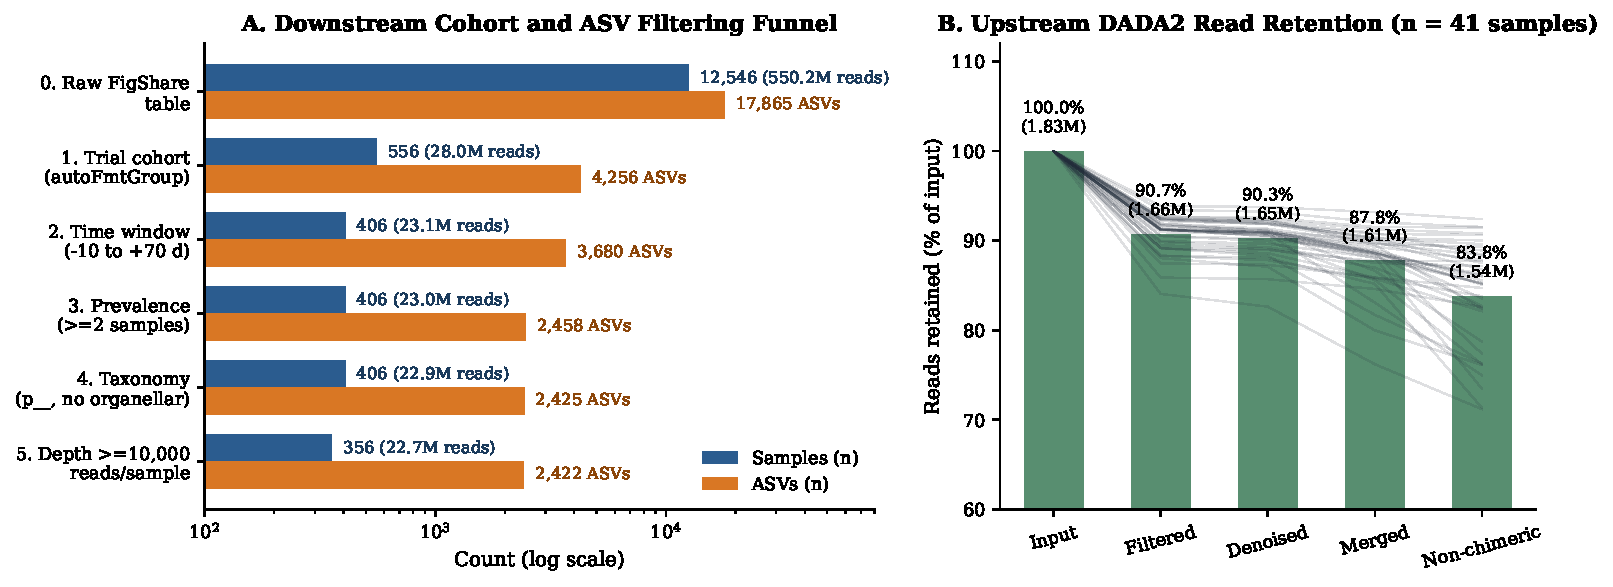
\includegraphics[width=\linewidth]{fig1_filtering_and_qc.pdf}
\caption{Cohort filtering funnel and upstream denoising retention. (\textbf{A}) Sample and ASV counts (log scale) and total sequencing reads across the six stages of the downstream filtering funnel (\texttt{00\_filtering\_funnel.tsv}). (\textbf{B}) Percentage and total count of input reads retained across sequential DADA2 denoising steps for the 41 upstream demonstration samples (\texttt{01\_dada2\_stats.tsv}); gray lines trace individual sample retention trajectories.}
\label{fig:filtering}
\end{figure}

\subsection{Cross-sectional alpha diversity comparisons and beta diversity ordination}
Pairwise Kruskal-Wallis tests on rarefied ASV richness (\texttt{observed\_features} at 10,000 reads/sample; $n = 356$ samples) across clinical and temporal groupings are summarized in Figure~\ref{fig:diversity}A. Across time categories relative to allo-HCT (\texttt{02\_kruskal\_categorical-time-relative-to-hct.tsv}), significant differences in observed ASVs were detected between \texttt{post} ($n = 225$) and \texttt{pre} ($n = 78$) samples ($H = 70.58$, $p = 4.42 \times 10^{-17}$, $q = 1.33 \times 10^{-16}$), between \texttt{peri} ($n = 53$) and \texttt{pre} ($n = 78$) samples ($H = 20.38$, $p = 6.36 \times 10^{-6}$, $q = 9.54 \times 10^{-6}$), and between \texttt{peri} ($n = 53$) and \texttt{post} ($n = 225$) samples ($H = 8.51$, $p = 0.00354$, $q = 0.00354$). When stratified by time categories relative to FMT (\texttt{02\_kruskal\_categorical-time-relative-to-fmt.tsv}), richness differed between \texttt{peri} ($n = 27$) and \texttt{post} ($n = 41$) samples ($H = 10.42$, $p = 0.00125$, $q = 0.00374$) and between \texttt{peri} ($n = 27$) and \texttt{pre} ($n = 288$) samples ($H = 5.87$, $p = 0.0154$, $q = 0.0231$), whereas no significant difference was observed between \texttt{post} ($n = 41$) and \texttt{pre} ($n = 288$) samples ($H = 1.58$, $p = 0.208$, $q = 0.208$).

In contrast, when all 356 samples were pooled across time points to compare the randomized intervention arms (\texttt{02\_kruskal\_autoFmtGroup.tsv}), observed ASV richness did not differ significantly between the control group ($n = 150$ samples) and the auto-FMT treatment group ($n = 206$ samples; $H = 1.29$, $p = 0.256$, $q = 0.256$; Figure~\ref{fig:diversity}A). Among clinical covariates, pairwise comparisons by stool consistency (\texttt{02\_kruskal\_Consistency.tsv}; $n = 355$ annotated samples) showed significant differences between \texttt{formed} ($n = 97$) and \texttt{semi-formed} ($n = 115$) stools ($H = 8.26$, $p = 0.00405$, $q = 0.0121$) and between \texttt{formed} ($n = 97$) and \texttt{liquid} ($n = 143$) stools ($H = 5.55$, $p = 0.0185$, $q = 0.0277$), but not between \texttt{liquid} and \texttt{semi-formed} stools ($H = 0.44$, $p = 0.507$, $q = 0.507$). Across stem cell graft sources (\texttt{02\_kruskal\_HCTSource.tsv}), significant differences were observed for unmodified bone marrow (\texttt{BM\_unmodified}, $n = 67$) versus unmodified peripheral blood stem cells (\texttt{PBSC\_unmodified}, $n = 128$; $H = 21.20$, $p = 4.14 \times 10^{-6}$, $q = 2.49 \times 10^{-5}$), \texttt{PBSC\_unmodified} ($n = 128$) versus T-cell depleted grafts (\texttt{TCD}, $n = 129$; $H = 18.86$, $p = 1.41 \times 10^{-5}$, $q = 4.22 \times 10^{-5}$), \texttt{BM\_unmodified} ($n = 67$) versus umbilical cord blood (\texttt{cord}, $n = 32$; $H = 10.30$, $p = 0.00133$, $q = 0.00266$), and \texttt{TCD} ($n = 129$) versus \texttt{cord} ($n = 32$; $H = 7.85$, $p = 0.00507$, $q = 0.00761$), whereas \texttt{BM\_unmodified} versus \texttt{TCD} ($H = 2.09$, $p = 0.149$, $q = 0.178$) and \texttt{PBSC\_unmodified} versus \texttt{cord} ($H = 0.013$, $p = 0.908$, $q = 0.908$) were not statistically significant.

In beta diversity PCoA ordinations (\texttt{05\_pcoa\_proportion\_explained.tsv}; Figure~\ref{fig:diversity}B), weighted UniFrac captured the highest proportion of variance along the first three principal coordinates (PC1 = 31.61\%, PC2 = 11.55\%, PC3 = 11.48\%; cumulative 54.64\%), followed by unweighted UniFrac (PC1 = 20.42\%, PC2 = 6.25\%, PC3 = 4.43\%; cumulative 31.10\%), Bray-Curtis dissimilarity (PC1 = 13.90\%, PC2 = 10.65\%, PC3 = 5.64\%; cumulative 30.19\%), and Jaccard distance (PC1 = 6.86\%, PC2 = 3.40\%, PC3 = 2.79\%; cumulative 13.05\%).

\begin{figure}[t]
\centering
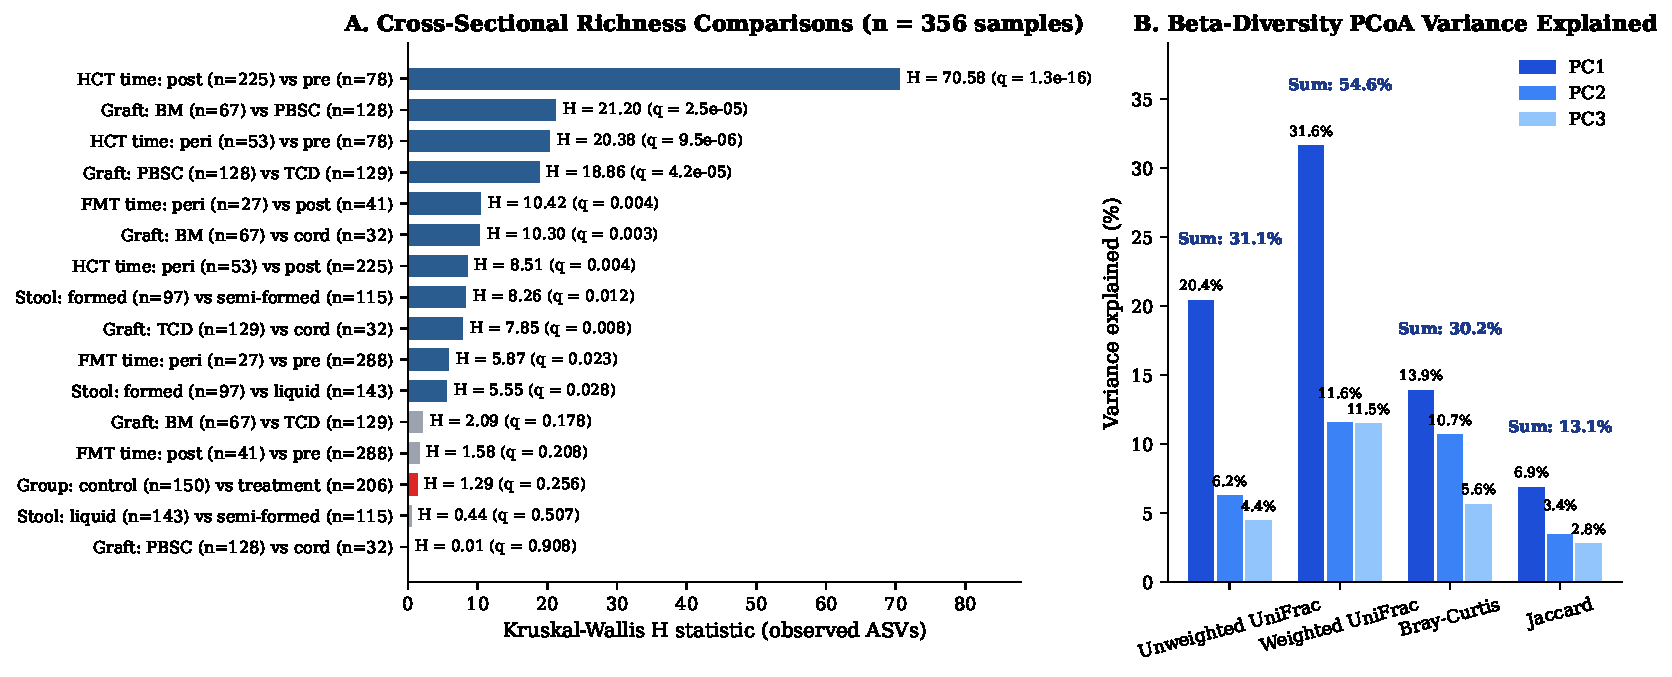
\includegraphics[width=\linewidth]{fig2_diversity_and_pcoa.pdf}
\caption{Cross-sectional alpha diversity comparisons and beta diversity ordination variance explained. (\textbf{A}) Pairwise Kruskal-Wallis $H$ statistics and Benjamini-Hochberg FDR-adjusted $q$-values for observed ASVs across temporal and clinical metadata groupings (\texttt{02\_kruskal\_*.tsv}); blue bars denote $q < 0.05$, gray bars denote $q \ge 0.05$, and the red bar highlights the pooled comparison between control and auto-FMT treatment groups ($H = 1.29$, $q = 0.256$). (\textbf{B}) Percentage of variance explained by the first three principal coordinates (PC1--PC3) across four beta diversity distance metrics (\texttt{05\_pcoa\_proportion\_explained.tsv}).}
\label{fig:diversity}
\end{figure}

\subsection{Longitudinal trajectory of microbial richness via linear mixed-effects modeling}
The linear mixed-effects (LME) model fit via REML evaluated \texttt{observed\_features} across 356 observations nested within 24 patients (2 to 34 observations per patient, mean 14.8; residual scale = 1,757.408, log-likelihood = $-1,840.587$; \texttt{03\_lme\_model\_summary.tsv}). Notably, the model summary recorded that the optimization algorithm did not converge (\texttt{Converged: No}).

Fixed- and random-effect parameter estimates from \texttt{03\_lme\_model\_results.tsv} are presented in Table~\ref{tab:lme} and Figure~\ref{fig:lme}. At day 0 relative to FMT, the baseline intercept for the control group was 65.687 observed ASVs ($\text{SE} = 6.696$, $z = 9.811$, $p < 0.001$, 95\% CI $[52.564, 78.810]$), and the main effect for the auto-FMT treatment group at day 0 was $+2.962$ ASVs ($\text{SE} = 8.849$, $z = 0.335$, $p = 0.738$, 95\% CI $[-14.381, 20.306]$). Across time (\texttt{day-relative-to-fmt}), the control group exhibited a statistically significant linear decline of $-0.859$ observed ASVs per day ($\text{SE} = 0.172$, $z = -5.003$, $p < 0.001$, 95\% CI $[-1.196, -0.523]$). The group-by-time interaction term (\texttt{day-relative-to-fmt:autoFmtGroup[T.treatment]}) was $+0.560$ observed ASVs per day ($\text{SE} = 0.232$, $z = 2.409$, $p = 0.016$, 95\% CI $[0.104, 1.015]$), corresponding to an implied net slope of $-0.299$ observed ASVs per day ($-0.859 + 0.560$) in the auto-FMT treatment group (Figure~\ref{fig:lme}A--B). The between-patient random intercept variance (\texttt{Group Var}) was 197.005 ($\text{SE} = 2.058$).

\begin{table}[t]
\centering
\footnotesize
\setlength{\tabcolsep}{3pt}
\caption{Linear mixed-effects (LME) model parameter estimates for \texttt{observed\_features} across 356 samples from 24 patients (\texttt{03\_lme\_model\_results.tsv} and \texttt{03\_lme\_model\_summary.tsv}; REML scale = 1,757.408, log-likelihood = $-1,840.587$, \texttt{Converged: No}).}
\label{tab:lme}
\begin{tabular}{lrrrrrr}
\toprule
Model term & Coef. & Std.\ Err. & $z$ & $P > |z|$ & 95\% CI low & 95\% CI high \\
\midrule
Intercept (Control at day 0) & 65.687 & 6.696 & 9.811 & $< 0.001$ & 52.564 & 78.810 \\
\texttt{autoFmtGroup[T.treatment]} & 2.962 & 8.849 & 0.335 & 0.738 & $-14.381$ & 20.306 \\
\texttt{day-relative-to-fmt} (Control) & $-0.859$ & 0.172 & $-5.003$ & $< 0.001$ & $-1.196$ & $-0.523$ \\
\texttt{day-relative-to-fmt:treatment} & 0.560 & 0.232 & 2.409 & 0.016 & 0.104 & 1.015 \\
\midrule
Patient random intercept (\texttt{Group Var}) & 197.005 & 2.058 & --- & --- & --- & --- \\
\bottomrule
\end{tabular}
\end{table}

\begin{figure}[t]
\centering
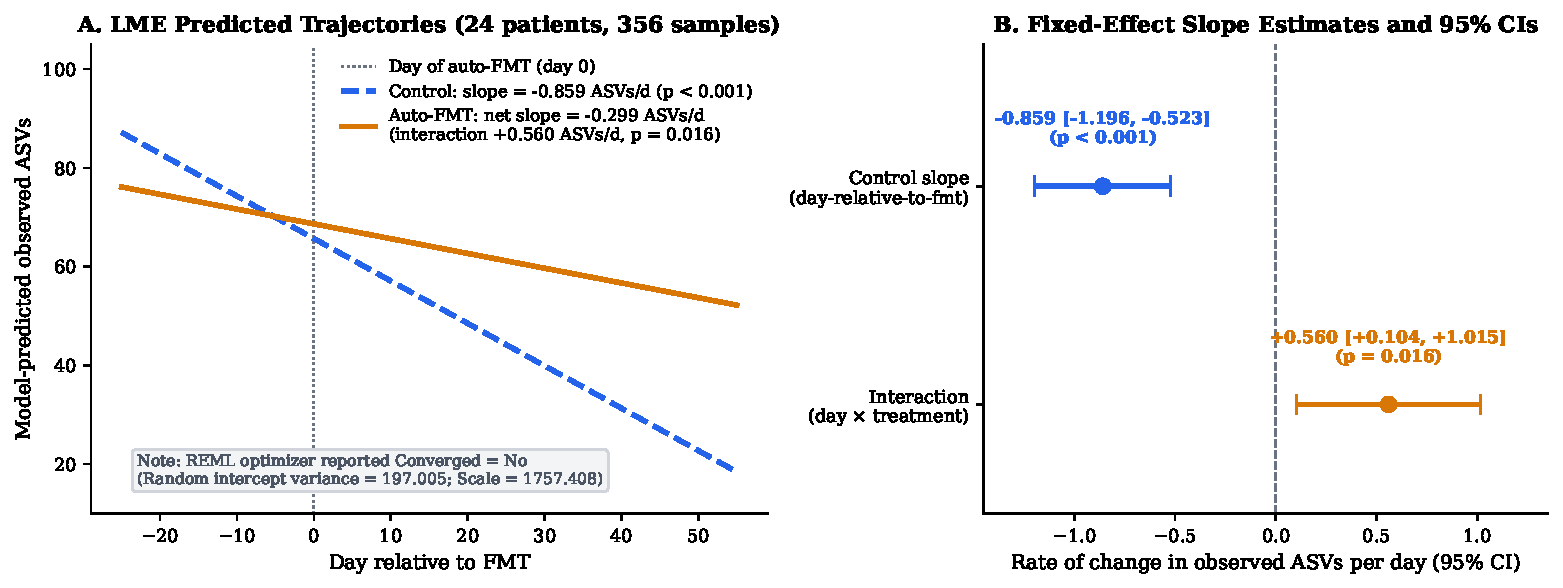
\includegraphics[width=\linewidth]{fig3_lme_trajectories.pdf}
\caption{Longitudinal linear mixed-effects (LME) model of observed ASV richness relative to FMT day. (\textbf{A}) Model-predicted linear trajectories of \texttt{observed\_features} for the control group (dashed blue line; slope $= -0.859$ ASVs/day) and the auto-FMT treatment group (solid orange line; implied net slope $= -0.299$ ASVs/day). (\textbf{B}) Point estimates and 95\% confidence intervals for the daily rate of change in the control group and the group-by-time interaction term (\texttt{03\_lme\_model\_results.tsv}).}
\label{fig:lme}
\end{figure}

\subsection{Temporal succession of microbial taxa predicted by random forest regression}
In the longitudinal feature volatility analysis (\texttt{04\_rf\_accuracy.tsv}), the random forest regressor trained on conditionally filtered genus-level relative frequencies predicted \texttt{week-relative-to-hct} with a mean squared error (MSE) of 4.249, Pearson correlation $r = 0.565$, coefficient of determination $R^2 = 0.319$, and $p = 2.37 \times 10^{-7}$ (linear fit slope $= 0.304$, standard error $= 0.053$, intercept $= 0.991$).

Twenty genus-level features met the prevalence ($\ge 10\%$ of samples) and abundance ($\ge 1\%$) thresholds and contributed to the random forest model (\texttt{04\_rf\_feature\_importance.tsv}; Figure~\ref{fig:rf}). The four highest-ranking features accounted for 40.92\% of total model importance: unclassified \textit{Enterococcaceae} (importance $= 0.124$), \textit{Clostridium} (family \textit{Clostridiaceae}; $0.109$), \textit{Enterococcaceae} genus \textit{Incertae Sedis} ($0.089$), and unclassified \textit{Lachnospiraceae} ($0.087$). Combined, the two \textit{Enterococcaceae} features accounted for 21.30\% of total importance, while the three \textit{Lachnospiraceae} features---unclassified \textit{Lachnospiraceae} ($0.087$), \textit{Murimonas} ($0.036$), and \textit{Sellimonas} ($0.033$)---accounted for 15.68\%. Additional features with importance scores above 0.030 included unclassified \textit{Actinobacteria} ($0.077$), unclassified \textit{Erysipelotrichaceae} ($0.061$), \textit{Tannockella} ($0.054$), unclassified \textit{Lactobacillaceae} ($0.047$), \textit{Streptococcus} ($0.046$), unclassified \textit{Bifidobacteriaceae} ($0.037$), \textit{Staphylococcus} ($0.035$), and \textit{Asaccharospora} ($0.035$), whereas \textit{Lactococcus} ($0.029$), unclassified \textit{Ruminococcaceae} ($0.026$), \textit{Akkermansia} ($0.023$), \textit{Veillonella} ($0.018$), \textit{Longicatena} ($0.017$), and \textit{Escherichia-Shigella} ($0.015$) each contributed less than 0.030 (Figure~\ref{fig:rf}).

\begin{figure}[t]
\centering
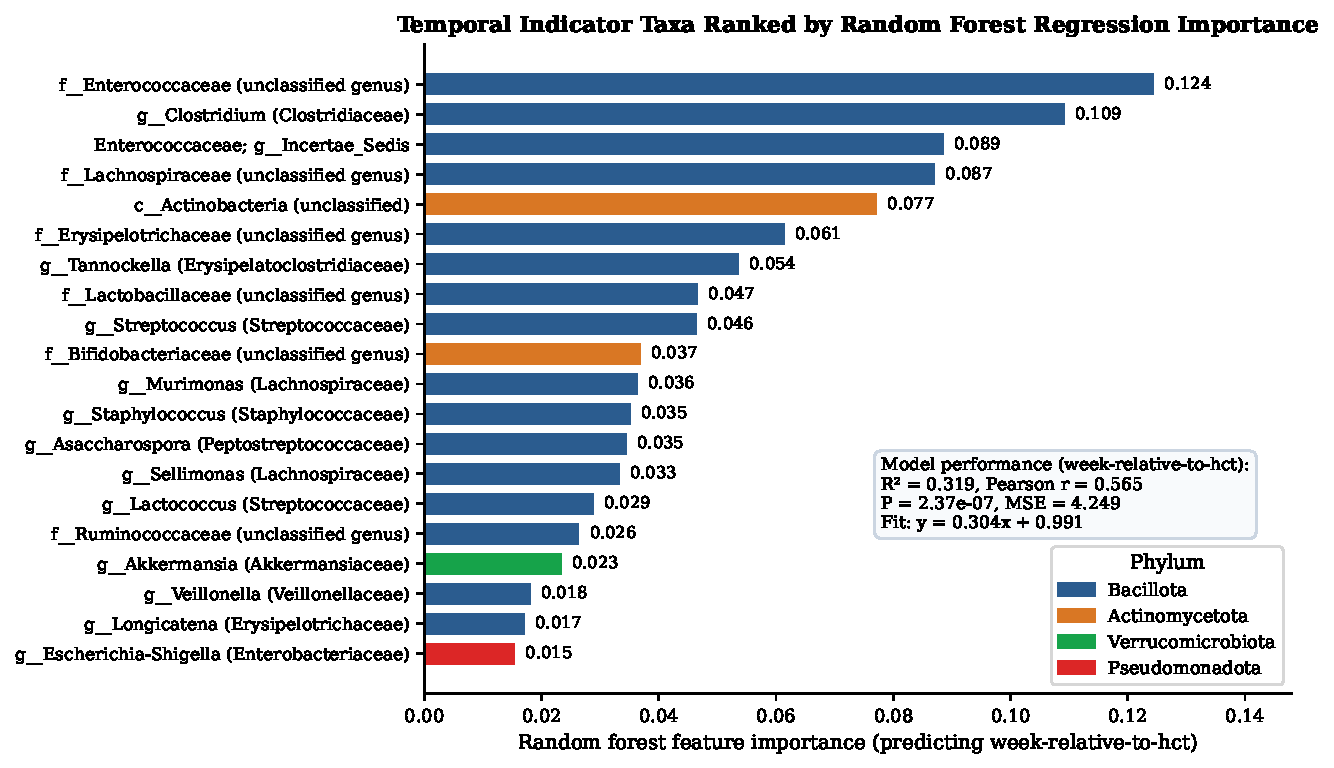
\includegraphics[width=0.92\linewidth]{fig4_rf_feature_importance.pdf}
\caption{Normalized feature importance scores of the 20 genus-level taxa retained in the random forest regression model predicting \texttt{week-relative-to-hct} (\texttt{04\_rf\_feature\_importance.tsv} and \texttt{04\_rf\_accuracy.tsv}). Bars are colored by bacterial phylum.}
\label{fig:rf}
\end{figure}

% 04-discussion.tex — Discussion, Limitations, and Conclusions
% Rule: Align claim strength with evidence (24 patients, LME non-convergence; avoid "prove", "demonstrate efficacy", "confirm"). Discuss all 6 limitations based on library/literature-matrix.md.

\section{Discussion}

\subsection{Principal findings}
Our longitudinal reanalysis of 356 fecal samples from 24 allo-HCT recipients illustrates how analytical model choice shapes the interpretation of clinical microbiome interventions. Across the cohort, transplantation was accompanied by a pronounced reduction in observed ASV richness between pre- and post-HCT time points ($H = 70.58$, $q = 1.33 \times 10^{-16}$), alongside substantial variation across stem cell graft sources and stool consistency categories. When all 356 samples were pooled across time in a cross-sectional Kruskal-Wallis test, no statistically significant difference in ASV richness was detected between the control ($n = 150$) and auto-FMT ($n = 206$) arms ($H = 1.29$, $p = 0.256$). In contrast, accounting for repeated within-patient measurements in a longitudinal linear mixed-effects (LME) model indicated a steep downward trajectory in the control group ($-0.859$ ASVs/day, $p < 0.001$) and a positive group-by-time interaction in the auto-FMT group ($+0.560$ ASVs/day, $p = 0.016$; implied net slope $-0.299$ ASVs/day), suggesting an attenuated rate of richness decline over the observation window. Concurrently, supervised random forest regression moderately predicted post-transplant week ($R^2 = 0.319$, $r = 0.565$, $p = 2.37 \times 10^{-7}$), identifying members of \textit{Enterococcaceae} (21.30\% combined importance across two features), \textit{Clostridium} (10.92\%), and \textit{Lachnospiraceae} (15.68\% combined across three features) as the primary taxa tracking temporal progression after allo-HCT.

The direction of the longitudinal interaction is consistent with the original trial, which reported that auto-FMT boosted microbial diversity \citep{taur2018reconstitution}. However, the original analysis included 25 patients, whereas our filtered reanalysis comprised 24 patients and 356 samples, and our single-slope LME on one richness index cannot by itself assess the compositional reestablishment described in that study.

\subsection{Comparison with previous methodological and clinical work}
The divergence between our null cross-sectional group comparison and the positive longitudinal interaction underscores a central principle in longitudinal microbiome research: pooling repeated observations across time conflates large within-subject temporal shifts with between-group treatment effects \citep{herman2024assessingb,zhang2026bayesian}. Because specimens collected from the same patient share host-specific baseline diversity and correlated temporal trajectories, treating all 356 samples as independent observations violates the exchangeability assumption of rank-based tests and allows the profound pre-to-post-HCT richness drop to obscure subtler differences in post-intervention recovery slopes \citep{herman2024assessingb,zhou2021linda}. In beta diversity ordinations, abundance-weighted phylogenetic distance (weighted UniFrac; PC1--PC3 cumulative variance 54.64\%) captured nearly twice the variation of presence/absence phylogenetic distance (unweighted UniFrac; 31.10\%) or non-phylogenetic Bray-Curtis dissimilarity (30.19\%), consistent with large shifts in dominant phylogenetic lineages---such as the post-transplant expansion of \textit{Enterococcaceae} and fluctuation of obligate anaerobic \textit{Clostridia} (\textit{Lachnospiraceae} and \textit{Clostridium})---driving community reorganization.

At the same time, recent methodological frameworks for fecal microbiota transplantation emphasize that neither alpha diversity recovery nor temporal shifts in taxonomic relative abundance are sufficient to establish donor microbiome engraftment \citep{herman2024assessing,herman2024assessingb}. As formalized by \citet{herman2024assessingb} and implemented in the QIIME 2 \texttt{q2-fmt} plugin \citep{herman2024assessing}, rigorous evaluation of FMT engraftment requires three complementary criteria: (1) chimeric asymmetric community coalescence, quantifying whether post-FMT recipient communities converge toward their specific baseline or donor reference profile over time; (2) donated microbiome indicator features, tracking the proportion of transferred donor features (such as Proportion of Engrafted Donated Features, PEDF) and differentially abundant taxa; and (3) temporal stability of the reconstituted community. Because our pipeline evaluated only cohort-level alpha diversity slopes and time-predictive genera without pairing post-FMT recipient profiles against each patient's own cryopreserved pre-antibiotic baseline, our findings reflect longitudinal richness retention and temporal succession rather than direct verification of autologous strain engraftment.

\subsection{Methodological limitations and future directions}
This reanalysis has six specific methodological limitations that temper clinical inference and motivate the adoption of specialized longitudinal microbiome tools:

\begin{enumerate}
  \item \textbf{Small sample size and unbalanced longitudinal design:} Although the analytical dataset comprised 356 fecal specimens, these observations were clustered within only 24 patients (10 control and 14 auto-FMT recipients), with per-patient sampling frequency ranging widely from 2 to 34 specimens (mean 14.8). This modest cohort size and irregular follow-up schedule limited statistical power and produced a wide 95\% confidence interval for the LME group-by-time interaction term ($0.104$ to $1.015$ ASVs/day, a nearly tenfold span). Future reanalyses should leverage estimation frameworks specifically designed for irregular, unbalanced longitudinal microbiome cohorts with missing visits \citep{barrera2025stochastic,fontaine2026locally}.
  \item \textbf{Non-convergence of the LME optimization algorithm:} The REML optimizer in \texttt{q2-longitudinal} reported non-convergence (\texttt{Converged: No}; residual scale $= 1,757.408$, patient random intercept variance $= 197.005$). In complex random-effects models for longitudinal microbiome data, estimation methods that rely on log-likelihood approximations are prone to biased estimates or unstable convergence \citep{barrera2025stochastic}. Consequently, the nominal $p = 0.016$ interaction effect must be interpreted cautiously as an exploratory trend rather than a definitive statistical conclusion. Applying a Stochastic Approximation Expectation-Maximization (SAEM) algorithm offers a more stable maximum likelihood estimation approach that directly accommodates unbalanced longitudinal designs without prior interpolation \citep{barrera2025stochastic}.
  \item \textbf{Oversimplification of pre- and post-FMT dynamics by a single linear slope:} Our LME specification fit a single constant linear slope across \texttt{day-relative-to-fmt} spanning days $-10$ to $+70$ relative to allo-HCT. Biologically, however, gut microbial richness undergoes a biphasic trajectory---rapid depletion during pre-FMT conditioning and antibiotic exposure followed by stabilization or recovery after auto-FMT reinfusion. Fitting one straight line across both phases averages pre-intervention injury with post-intervention recovery; thus, the net slope in the auto-FMT arm remained slightly negative ($-0.299$ ASVs/day) despite a positive interaction term ($+0.560$ ASVs/day). Piecewise (broken-stick) mixed models or locally sparse varying coefficient mixed models (LSVCMM), which exploit penalized kernel smoothing and random effects for serial correlation to identify specific time intervals of significant group differences \citep{fontaine2026locally}, would better match the underlying clinical timeline.
  \item \textbf{Sample loss and sampling variance from single-step rarefying:} Enforcing a uniform rarefying threshold of 10,000 reads per sample (\texttt{core-metrics-phylogenetic}) excluded 50 of the 406 in-window samples (12.32\%) and discarded excess sequencing reads from deeper libraries. As demonstrated by \citet{mcmurdie2013waste}, single rarefying is statistically inadmissible because it discards valid information and inflates Type-II error rates; moreover, in allo-HCT cohorts, low-depth specimens may disproportionately represent severe post-antibiotic bacterial depletion, introducing potential selection bias. Within the QIIME 2 ecosystem, replacing single rarefying with bootstrapped or multi-rarefaction diversity averaging via \texttt{q2-boots} \citep{raspet2024facilitating} would incorporate all valid sequence data and quantify subsampling uncertainty.
  \item \textbf{Pseudoreplication in cross-sectional rank tests:} The pairwise Kruskal-Wallis comparisons treated 356 correlated observations from 24 patients as independent samples. Ignoring within-subject correlation in repeated-measures microbiome data is known to distort type I and type II error rates \citep{herman2024assessingb,zhou2021linda,zhang2026bayesian}. Cross-sectional rank tests should therefore be restricted to single-time-point summaries (e.g., baseline or a fixed landmark week) or replaced by mixed-effects models that explicitly partition within- and between-subject variance.
  \item \textbf{Temporal prediction versus therapeutic engraftment and compositional bias:} In our feature volatility analysis, random forest regression was trained on genus-level relative frequencies to predict \texttt{week-relative-to-hct} ($R^2 = 0.319$), without stratifying by treatment arm or correcting for compositional bias. Consequently, top-ranked taxa such as \textit{Enterococcaceae} and \textit{Lachnospiraceae} represent markers of time since transplantation rather than biomarkers of auto-FMT efficacy. Furthermore, because amplicon sequencing yields compositional relative abundances with high zero inflation, future analyses should apply centered log-ratio (CLR) linear mixed models with mode-based bias correction (\texttt{LinDA-LMM}) \citep{zhou2021linda} or Bayesian nonparametric longitudinal factor models (\texttt{LODI}) \citep{zhang2026bayesian} to test group-by-time differential abundance while accounting for dynamic microbial co-abundance networks.
\end{enumerate}

\subsection{Conclusions}
In this longitudinal QIIME 2 reanalysis of 24 allo-HCT patients (356 fecal samples), gut microbial richness declined sharply after transplantation, and supervised random forest regression identified \textit{Enterococcaceae}, \textit{Clostridium}, and \textit{Lachnospiraceae} as key indicators of post-transplant temporal succession ($R^2 = 0.319$). While pooled cross-sectional Kruskal-Wallis testing showed no difference between randomized arms ($p = 0.256$), longitudinal LME modeling detected a slower rate of richness decline in the auto-FMT group ($+0.560$ ASVs/day interaction, $p = 0.016$). However, because the cohort was small and unbalanced, the LME optimizer did not converge, a single linear slope was fit across pre- and post-FMT windows, and donor strain coalescence was not directly evaluated, these results should be viewed as methodological and exploratory rather than conclusive evidence of clinical efficacy. Incorporating multi-rarefaction diversity (\texttt{q2-boots}), patient-baseline coalescence metrics (\texttt{q2-fmt}), stochastic mixed-model estimation (SAEM), time-varying coefficient models (LSVCMM), and compositionally adjusted longitudinal differential abundance (\texttt{LinDA-LMM}) will be essential for robust inference in future microbiome intervention trials.

% 07-declarations.tex — Declarations
% Rule: Author contributions, Competing interests, and Funding must only be completed by the authors; keep [To be completed by the authors.].

\section*{Data availability}
The 16S rRNA gene amplicon sequencing data and clinical metadata reanalyzed in this study originate from ClinicalTrials.gov NCT02269150 and are publicly available through the QIIME 2 Cancer Microbiome Intervention Tutorial (\url{https://docs.qiime2.org/jupyterbooks/cancer-microbiome-intervention-tutorial/}). Processed summary tables and statistical outputs used to generate all tables and figures in this manuscript are provided in \texttt{data/tables/}.

\section*{Code availability}
The complete QIIME 2 bioinformatics and longitudinal analysis workflow is available in \texttt{data/Qiime2\_Pipeline.sh}, and the Python script used to reproduce Figures 1--4 from the summary tables is available in \texttt{manuscript/plot\_figures.py}.

\section*{Ethics statement}
This work is a secondary computational reanalysis of publicly available, de-identified human microbiome sequencing data from a previously published clinical trial (NCT02269150). No new human participants were recruited and no identifiable private information was accessed; therefore, additional institutional review board approval was not required.

\section*{Author contributions}
[To be completed by the authors.]

\section*{Competing interests}
[To be completed by the authors.]

\section*{Funding}
[To be completed by the authors.]

\section*{Use of AI tools}
An AI coding and research assistant (Google Antigravity) was used to assist with searching arXiv literature via the \texttt{arxiv} and \texttt{paper-library} skills, organizing reading notes and the literature comparison matrix (\texttt{library/literature-matrix.md}), writing the Python figure-plotting script (\texttt{manuscript/plot\_figures.py}), and drafting and formatting the English LaTeX manuscript (\texttt{manuscript/sections/*.tex}). All numerical values, statistical test outputs, software parameters, and verbatim literature quotations were cross-checked against the primary data tables (\texttt{data/tables/*.tsv}), pipeline script (\texttt{data/Qiime2\_Pipeline.sh}), and downloaded PDF articles (\texttt{papers/*.pdf}).


\bibliographystyle{plainnat}
\bibliography{references}

\end{document}
